\label{chap:4}
\section{Simulação}\label{sec:simulation}

Simulamos a resposta de frequência de uma sala utilizando o algoritmo Image-Source Model \cite{simulation}.

A sala utilizada nas simulações tem dimensões $4,45m \times 3,55m \times 2,5m$ (largura × comprimento × altura) e é completamente selada. Além disso, o coeficiente de absorção de todas as suas paredes é o mesmo, considerando que todas são feitas do mesmo material. O material utilizado altera o tempo de reverberação, sendo que o algoritmo de simulação calcula o coeficiente de absorção das paredes da sala dependendo do tempo de reverberação escolhido. O arranjo de microfones é linear e foi posicionado em torno do ponto $\mathpzc{Mic_c = [2 1,5 1,6]^T}$. Foi simulado apenas o cenário com 2 microfones e 2 fontes. As fontes foram distribuídas em torno do centro do arranjo, com dois parâmetros para identificá-las: o DOA de cada uma, e a distância delas até o arranjo. O parâmetro mais importante da sala é o tempo de reverberação. O tempo utilizado nesta dissertação é o ${T_{60}}$, que é o tempo requerido para que a energia das componentes relativas a reflexões do sinal caia a 60 dB abaixo do nível do som direto.

As fontes utilizadas foram do SASSEC, correspondendo a trechos de sinais de voz de 10 segundos de duração cada, amostrados a 16 kHz. Decimamos os sinais para que a frequência de amostragem fosse reduzida para 8 kHz. As informações do ambiente simulado são dadas na Figura \ref{fig:environment}.

\begin{figure}
    \centering
    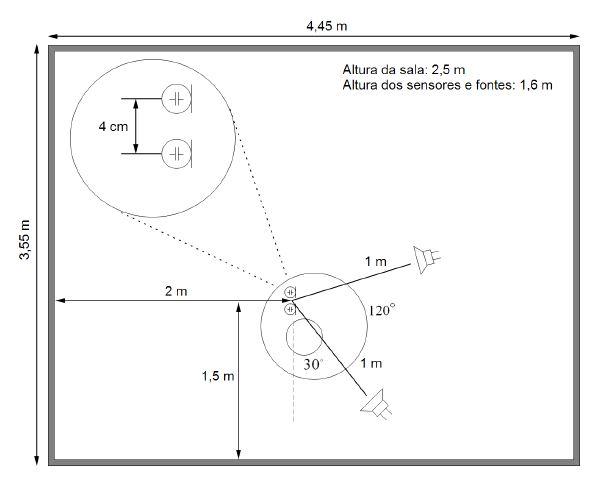
\includegraphics{environment.JPG}
    \caption{Configuração da sala utilizada nos testes.}
    \label{fig:environment}
\end{figure}


 \section{Análise dos Algoritmos}\label{sec:analysis}
    
    Nas condições de simulação descritas na Seção \ref{sec:simulation}, comparamos os métodos ICA-EBM e Natural ICA em relação aos resultados e à performance quanto à separação dos sinais. Vale ressaltar que o objetivo destes experimentos foi avaliar unicamente a etapa de separação dos sinais e, por isso, não houve qualquer alteração no método de resolução da permutação e de escalonamento.  Inicialmente, a simulalação foi feita com tempo de reverberação $\mathpzc{T_{60}}$ igual a 0,1s. Neste cenário, os sinais das fontes e dos sensores são mostrados nas Figuras \ref{fig:sources} e \ref{fig:sensors}, respectivamente.
    
    Após aplicar a STFT (definida na Seção \ref{sec:stft}) para transformar os sinais para o domínio da frequência e fazer a separação das fontes, incluindo tanto a etapa de pré-processamento (descrita na Seção \ref{sec:whitening}) quanto a de pós-processamento (apresentada na Seção \ref{sec:tdoa}), obtivemos as estimativas das fontes mostradas nas Figuras \ref{fig:icaebm} e \ref{fig:natica} para os métodos ICA-EBM e Natural ICA, respectivamente.
    
    Analisando os resultados, podemos concluir que ambos os métodos geraram boas estimativas. Isto pode ser facilmente observado nos gráficos das estimativas das fontes mostrados nas Figuras \ref{fig:icaebm} e \ref{fig:natica} . Entretanto, o algoritmo ICA-EBM levou consideravelmente mais tempo para obtenção do resultado que o algoritmo Natural ICA associado ao FastICA. Conforme aumentamos o tempo de reverberação $\mathpzc{T_{60}}$ do ambiente de simulação, ambos os métodos passaram a ter suas estimativas degradadas, mas ainda assim, se mantiveram bem próximos. Nas Figuras \ref{fig:natica} e \ref{fig:icaebm} são apresentados os valores da SIR, SAR e SDR obtidos com os algoritmos Natural ICA + FastICA e ICA-EBM, respectivamente, para diferentes tempos de reverberação. Pode-se observar destas figuras que o algoritmo ICA-EBM apresenta um desempenho ligeiramente superior ao do Natural ICA + FastICA, no entanto com convergência mais lenta.
    
    \begin{figure}
        \centering
        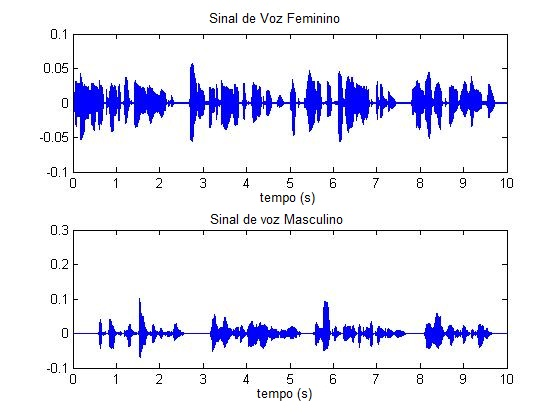
\includegraphics[scale=0.7]{sources.jpg}
            \caption{Sinais de cada uma das fontes no domínio do tempo.}
        \label{fig:sources}
        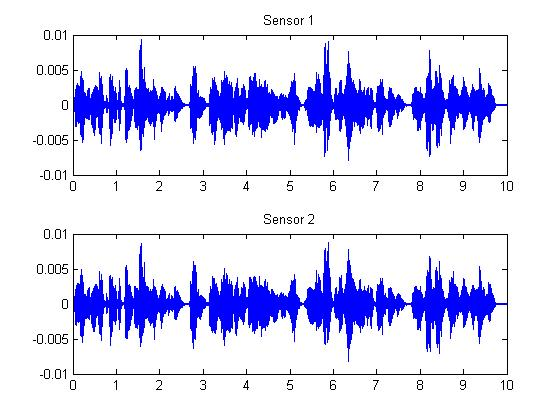
\includegraphics[scale=0.7]{sensors.jpg}
            \caption{Sinais em cada um dos sensores no domínio do tempo para $\mathpzc{T_{60}}$ = 0.1s.}
        \label{fig:sensors}
    \end{figure}
    
    \begin{figure}
        \centering
        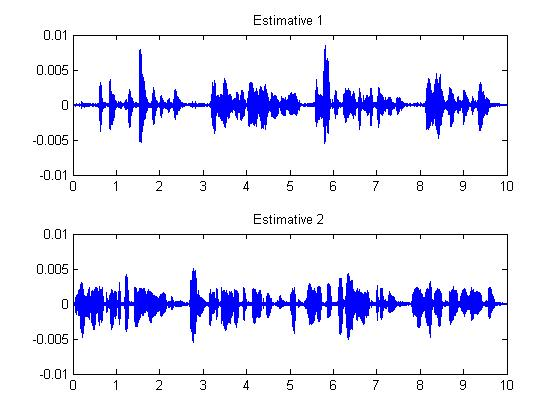
\includegraphics[scale=0.7]{estimatives_FASTICA.jpg}
        \caption{Sinais de estimativa das fontes obtidas pelo algoritmo ICA-EBM no domínio do tempo para $\mathpzc{T_{60}}$ = 0.1s.}
        \label{fig:icaebm}
        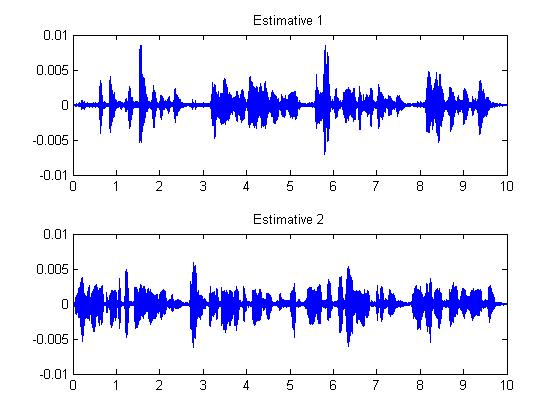
\includegraphics[scale=0.7]{estimatives_NATICA.jpg}
        \caption{Sinais de estimativa das fontes obtidas pelo algoritmo Natural ICA + FastICA  no domínio do tempo para $\mathpzc{T_{60}}$ = 0.1s.}
        \label{fig:natica}
    \end{figure}
    
    
    \begin{figure}
        \centering
        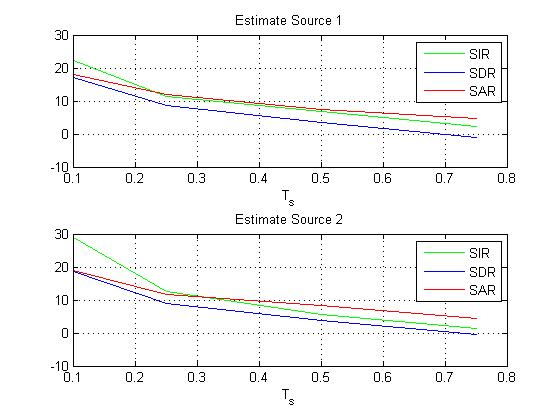
\includegraphics[scale=0.7]{resultTsnaturalica.jpg}
        \caption{Métricas de desempenho em função do tempo de reverberação $\mathpzc{T_{60}}$ para o algoritmo Natural ICA + FastICA.}
        \label{fig:T60natica}
         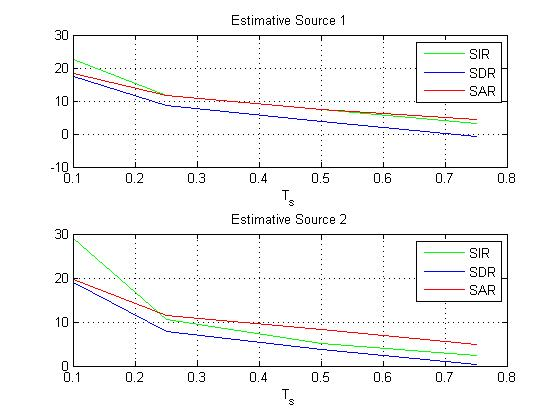
\includegraphics[scale=0.7]{resultTsicaebm.jpg}
        \caption{Métricas de desempenho em função do tempo de reverberação $\mathpzc{T_{60}}$ para o algoritmo ICA-EBM.}
        \label{fig:T60icaebm}
    \end{figure}
    